\documentclass{tufte-book}
\usepackage[french]{babel}
\usepackage[utf8]{inputenc}

\hypersetup{colorlinks}% uncomment this line if you prefer colored hyperlinks (e.g., for onscreen viewing)

%%
% Book metadata
\title{Vim - Le guide pour les êtres humains\thanks{Merci à la communauté Vim.}}
\author[Vincent Jousse]{Vincent\ Jousse}
\publisher{Vincent Jousse}

%%
% If they're installed, use Bergamo and Chantilly from www.fontsite.com.
% They're clones of Bembo and Gill Sans, respectively.
%\IfFileExists{bergamo.sty}{\usepackage[osf]{bergamo}}{}% Bembo
%\IfFileExists{chantill.sty}{\usepackage{chantill}}{}% Gill Sans

%\usepackage{microtype}

%%
% Just some sample text
\usepackage{lipsum}

%%
% For nicely typeset tabular material
\usepackage{booktabs}

%%
% For graphics / images
\usepackage{graphicx}
\setkeys{Gin}{width=\linewidth,totalheight=\textheight,keepaspectratio}
\graphicspath{{graphics/}}

% The fancyvrb package lets us customize the formatting of verbatim
% environments.  We use a slightly smaller font.
\usepackage{fancyvrb}
\fvset{fontsize=\normalsize}

%%
% Prints argument within hanging parentheses (i.e., parentheses that take
% up no horizontal space).  Useful in tabular environments.
\newcommand{\hangp}[1]{\makebox[0pt][r]{(}#1\makebox[0pt][l]{)}}

%%
% Prints an asterisk that takes up no horizontal space.
% Useful in tabular environments.
\newcommand{\hangstar}{\makebox[0pt][l]{*}}

%%
% Prints a trailing space in a smart way.
\usepackage{xspace}

% Format code using pygment
\usepackage{minted}
\usemintedstyle{solarized}
%\definecolor{bg}{RGB}{0,43,54}
%Light bg
\definecolor{bg}{RGB}{253,246,227}

%%
% Some shortcuts for Tufte's book titles.  The lowercase commands will
% produce the initials of the book title in italics.  The all-caps commands
% will print out the full title of the book in italics.
\newcommand{\vdqi}{\textit{VDQI}\xspace}
\newcommand{\ei}{\textit{EI}\xspace}
\newcommand{\ve}{\textit{VE}\xspace}
\newcommand{\be}{\textit{BE}\xspace}
\newcommand{\VDQI}{\textit{The Visual Display of Quantitative Information}\xspace}
\newcommand{\EI}{\textit{Envisioning Information}\xspace}
\newcommand{\VE}{\textit{Visual Explanations}\xspace}
\newcommand{\BE}{\textit{Beautiful Evidence}\xspace}

\newcommand{\TL}{Tufte-\LaTeX\xspace}

% Prints the month name (e.g., January) and the year (e.g., 2008)
\newcommand{\monthyear}{%
  \ifcase\month\or January\or February\or March\or April\or May\or June\or
  July\or August\or September\or October\or November\or
  December\fi\space\number\year
}

% Prints an epigraph and speaker in sans serif, all-caps type.
\newcommand{\openepigraph}[2]{%
  %\sffamily\fontsize{14}{16}\selectfont
  \begin{fullwidth}
  \sffamily\large
  \begin{doublespace}
  \noindent\allcaps{#1}\\% epigraph
  \noindent\allcaps{#2}% author
  \end{doublespace}
  \end{fullwidth}
}

% Inserts a blank page
\newcommand{\blankpage}{\newpage\hbox{}\thispagestyle{empty}\newpage}

\usepackage{units}

% Typesets the font size, leading, and measure in the form of 10/12x26 pc.
\newcommand{\measure}[3]{#1/#2$\times$\unit[#3]{pc}}

% Macros for typesetting the documentation
\newcommand{\hlred}[1]{\textcolor{Maroon}{#1}}% prints in red
\newcommand{\hangleft}[1]{\makebox[0pt][r]{#1}}
\newcommand{\hairsp}{\hspace{1pt}}% hair space
\newcommand{\hquad}{\hskip0.5em\relax}% half quad space
\newcommand{\TODO}{\textcolor{red}{\bf TODO!}\xspace}
\newcommand{\ie}{\textit{i.\hairsp{}e.}\xspace}
\newcommand{\eg}{\textit{e.\hairsp{}g.}\xspace}
\newcommand{\na}{\quad--}% used in tables for N/A cells
\providecommand{\XeLaTeX}{X\lower.5ex\hbox{\kern-0.15em\reflectbox{E}}\kern-0.1em\LaTeX}
\newcommand{\tXeLaTeX}{\XeLaTeX\index{XeLaTeX@\protect\XeLaTeX}}
% \index{\texttt{\textbackslash xyz}@\hangleft{\texttt{\textbackslash}}\texttt{xyz}}
\newcommand{\tuftebs}{\symbol{'134}}% a backslash in tt type in OT1/T1
\newcommand{\doccmdnoindex}[2][]{\texttt{\tuftebs#2}}% command name -- adds backslash automatically (and doesn't add cmd to the index)
\newcommand{\doccmddef}[2][]{%
  \hlred{\texttt{\tuftebs#2}}\label{cmd:#2}%
  \ifthenelse{\isempty{#1}}%
    {% add the command to the index
      \index{#2 command@\protect\hangleft{\texttt{\tuftebs}}\texttt{#2}}% command name
    }%
    {% add the command and package to the index
      \index{#2 command@\protect\hangleft{\texttt{\tuftebs}}\texttt{#2} (\texttt{#1} package)}% command name
      \index{#1 package@\texttt{#1} package}\index{packages!#1@\texttt{#1}}% package name
    }%
}% command name -- adds backslash automatically
\newcommand{\doccmd}[2][]{%
  \texttt{\tuftebs#2}%
  \ifthenelse{\isempty{#1}}%
    {% add the command to the index
      \index{#2 command@\protect\hangleft{\texttt{\tuftebs}}\texttt{#2}}% command name
    }%
    {% add the command and package to the index
      \index{#2 command@\protect\hangleft{\texttt{\tuftebs}}\texttt{#2} (\texttt{#1} package)}% command name
      \index{#1 package@\texttt{#1} package}\index{packages!#1@\texttt{#1}}% package name
    }%
}% command name -- adds backslash automatically
\newcommand{\docopt}[1]{\ensuremath{\langle}\textrm{\textit{#1}}\ensuremath{\rangle}}% optional command argument
\newcommand{\docarg}[1]{\textrm{\textit{#1}}}% (required) command argument
\newenvironment{docspec}{\begin{quotation}\ttfamily\parskip0pt\parindent0pt\ignorespaces}{\end{quotation}}% command specification environment
\newcommand{\docenv}[1]{\texttt{#1}\index{#1 environment@\texttt{#1} environment}\index{environments!#1@\texttt{#1}}}% environment name
\newcommand{\docenvdef}[1]{\hlred{\texttt{#1}}\label{env:#1}\index{#1 environment@\texttt{#1} environment}\index{environments!#1@\texttt{#1}}}% environment name
\newcommand{\docpkg}[1]{\texttt{#1}\index{#1 package@\texttt{#1} package}\index{packages!#1@\texttt{#1}}}% package name
\newcommand{\doccls}[1]{\texttt{#1}}% document class name
\newcommand{\docclsopt}[1]{\texttt{#1}\index{#1 class option@\texttt{#1} class option}\index{class options!#1@\texttt{#1}}}% document class option name
\newcommand{\docclsoptdef}[1]{\hlred{\texttt{#1}}\label{clsopt:#1}\index{#1 class option@\texttt{#1} class option}\index{class options!#1@\texttt{#1}}}% document class option name defined
\newcommand{\docmsg}[2]{\bigskip\begin{fullwidth}\noindent\ttfamily#1\end{fullwidth}\medskip\par\noindent#2}
\newcommand{\docfilehook}[2]{\texttt{#1}\index{file hooks!#2}\index{#1@\texttt{#1}}}
\newcommand{\doccounter}[1]{\texttt{#1}\index{#1 counter@\texttt{#1} counter}}

% Keys shortcuts
\newcommand{\tesc}{\hlred{Esc} (\hlred{Échap})\xspace}
\newcommand{\ttesc}{la touche \tesc}
\newcommand{\tshift}{\hlred{Shift}\xspace}
\newcommand{\ttshift}{la touche \tshift}
\newcommand{\ti}{\hlred{i}\xspace}
\newcommand{\tti}{la touche \ti}
\newcommand{\ttm}{la touche \hlred{m}\xspace}
\newcommand{\tto}{la touche \hlred{o}\xspace}
\newcommand{\tp}{\hlred{p}\xspace}
\newcommand{\ttp}{la touche \tp}
\newcommand{\tv}{\hlred{v}\xspace}
\newcommand{\ttv}{la touche \tv}
\newcommand{\ty}{\hlred{y}\xspace}
\newcommand{\tty}{la touche \ty}

\newcommand{\vimscmd}[1]{\fcolorbox{black}{bg}{\hlred{\Verb|{\footnotesize #1}|}}}
\newcommand{\vimcmd}[1]{\fcolorbox{black}{bg}{\hlred{\Verb|#1|}}}

\newcommand{\scmd}[1]{\fcolorbox{black}{white}{\hlred{\Verb|{\footnotesize #1}|}}}
\newcommand{\ncmd}[1]{\fcolorbox{black}{white}{\hlred{\Verb|#1|}}}

\newcommand{\vim}{\emph{Vim}\xspace}
\newcommand{\vimrc}{\emph{.vimrc}\xspace}


% Generates the index
\usepackage{makeidx}
\makeindex


\begin{document}

% Front matter
\frontmatter

% r.1 blank page
\blankpage

% r.3 full title page
\maketitle


% v.4 copyright page
\newpage
\begin{fullwidth}
~\vfill
\thispagestyle{empty}
\setlength{\parindent}{0pt}
\setlength{\parskip}{\baselineskip}
Copyright \copyright\ \the\year\ \thanklessauthor

\par\smallcaps{Publié par \thanklesspublisher}

\par\smallcaps{Style \LaTeX{} \url{http://tufte-latex.googlecode.com}}

\par Si vous n'avez pas payé cette copie, bah tant pis pour moi ;) Mais sachez que vous auriez dû !

\end{fullwidth}

% r.5 contents
\tableofcontents

\listoffigures

\listoftables

% r.7 dedication
\cleardoublepage
~\vfill
\begin{doublespace}
\noindent\fontsize{18}{22}\selectfont\itshape
\nohyphenation
Merci à ma femme et mes enfants qui ont permis à ce livre de voir le jour.
\end{doublespace}
\vfill
\vfill

% r.9 introduction
\cleardoublepage

\chapter*{Introduction}

\newthought{Lorsque le besoin} d'écrire ou de coder se fait se sentir, le choix d'un éditeur de texte est primordial. Il en existe énormément sur le "marché", mais peu d'entre eux peuvent se targuer d'environ 40 ans d'existence. C'est le cas d'\emph{Emacs} (\url{http://www.gnu.org/software/emacs/}), de \emph{Vi} et de son "successeur amélioré" \vim (\url{http://www.vim.org/}). Ils ont été créés dans les années 70 et sont toujours très utilisés actuellement. Comme vous avez sans doute pu le voir, ce n'est pas grâce à la beauté de leur site internet ou à l'efficacité de leur communication. Voici quelques \textbf{raisons de leur succès} :

\begin{description}
    \item[Pour la vie] \hfill \\ Ils s'apprennent une fois et s'utilisent pour toujours. Dans un monde où les technologies/langages changent tout le temps, c'est une aubaine de pouvoir investir sur du long terme.
    \item[Partout] \hfill \\ Ils sont disponibles sur toutes les plateformes possibles et imaginables (et l'ont toujours été).
    \item[Augmentent votre vitesse d'édition de texte] \hfill \\ Grâce à leurs particularités (notamment l'utilisation du clavier), ils permettent d'éditer du texte très rapidement.
    \item[Couteaux suisses] \hfill \\ Ils permettent d'éditer tout et n'importe quoi. Quand vous changerez de langage de programmation, vous n'aurez pas à changer d'éditeur. À noter que ce livre a bien sûr été écrit avec \vim.
\end{description}

Et pourtant, ces éditeurs de texte restent difficiles à apprendre. Non pas qu'ils soient plus compliqués qu'autre chose, non pas que vous ne soyez pas à la hauteur, mais plutôt à cause d'un manque de pédagogie des différentes documentations.

Ce livre a pour but de pallier ce manque en vous guidant tout au long de votre découverte de \vim\sidenote{Je laisse \emph{Emacs} à ceux qui savent. Pour un bref comparatif c'est ici : \url{http://fr.wikipedia.org/wiki/Guerre_d'\%C3\%A9diteurs}. Les goûts et les couleurs …}. Il ne prétend pas être un guide exhaustif, vous pouvez essayer \emph{A Byte of \vim} pour celà : \url{http://www.swaroopch.org/notes/Vim}. En revanche, il prétend diminuer la marche à franchir pour s'habituer à \vim. À mon sens, le plus compliqué avec \vim, c'est de ne pas se décourager de suite et de trouver une méthode qui vous permette de l'apprendre au fur et à mesure. Nous avons tous un travail à effectuer au quotidien, et perdre toute sa productivité à cause d'un changement d'éditeur de texte n'est pas envisageable.

Vous trouverez beaucoup de personnes pour vous dire \og mais tu n'as qu'à t'y mettre pour de bon \fg, \og tu verras après ça va aller mieux \fg, certes, mais vous devez toujours être productif au jour le jour, ça ne change rien au problème. L'approche de ce livre est la suivante :

\begin{enumerate}
    \item Disposer d'un \vim un temps soit peu moderne : coloration syntaxique et jolies couleurs.
    \item Pouvoir utiliser \vim comme n'importe quel autre éditeur de texte : éditer facilement du code et naviguer entre les fichiers en utilisant la souris.
    \item Apprendre des raccourcis clavier et se passer de la souris au fur et à mesure.
    \item Installer un \emph{best-of} des plugins pour commencer à tirer partie de la puissance de \vim.
\end{enumerate}

À partir du point numéro 2, vous pourrez déjà utiliser \vim au quotidien sans perdre énormément de productivité. Et c'est là que la différence se fait : si vous pouvez intégrer \vim dans votre quotidien c'est gagné. Vous aurez ensuite toute votre vie pour connaître tous les raccourcis clavier.

Vous aussi vous en avez marre d'attendre la release de TextMate 2\footnote{À noter que depuis l'écriture de ce livre, le code de TextMate 2 a été publié sous licence GPL : \url{https://github.com/textmate/textmate}} ? D'essayer le n-ième éditeur à la mode et de devoir tout réapprendre et ce jusqu'à la prochaine mode ? De devoir changer d'éditeur quand vous passez de votre Mac, à votre Windows, à votre Linux ? Alors vous aussi, rejoignez la communauté des gens heureux de leur éditeur de texte. \textbf{Le changement, c'est maintenant} !

\section{Pour qui ?}

\newthought{Toute personne} étant amenée à produire du texte (code, livre, rapports, présentations, ...) de manière régulière. Les développeurs sont bien sûr une cible privilégiée, mais pas uniquement.

Par exemple vous êtes :
\begin{description}
    \item[Étudiant] Si vous voulez faire bien sur un CV, c'est un must (en plus d'être un attrape geekette en puissance\footnote{À confirmer.}). Vous aurez un outil unique pour écrire tout ce que vous avez à écrire (et que vous pourrez réutiliser tout au long de votre carrière) : vos rapports en \LaTeX, vos présentations\footnote{En utilisant \emph{impress.js} par exemple : \url{http://bartaz.github.com/impress.js}. Basé sur du HTML/JS/CSS, je vous le recommande grandement pour des présentations originales et basées sur des technologies non propriétaires.}, votre code (si vous avez besoin d'OpenOffice ou de Word pour écrire vos rapports, il est temps de changer d'outil et d'utiliser \LaTeX).
    \item[Enseignant] Il est temps de montrer l'exemple et d'apprendre à vos étudiants à bien utiliser un des outils qui leur servira à vie, bien plus qu'un quelconque langage de programmation.
    \item[Codeur] Investir dans votre outil de tous les jours est indispensable. Quitte à apprendre des raccourcis claviers, autant le faire de manière utile. Si cet investissement est encore rentable dans 10 ans, c'est ce que l'on pourrait appeler l'investissement parfait, c'est \vim.
    \item[Administrateur système Unix] Si vous utilisez \emph{Emacs} vous êtes pardonnable. Si vous utilisez nano/pico je ne peux plus rien pour vous, sinon il est grand temps de s'y mettre les gars. Administrer un système Unix à distance est un des cas d'utilisation parfait pour \vim (un éditeur de texte surpuissant ne nécessitant pas d'interface graphique).
    \item[Écrivain] Si vous écrivez en markdown/reStructuredText/WikiMarkup ou en \LaTeX, \vim vous fera gagner beaucoup de temps. Vous ne pourrez plus repasser à un autre éditeur, ou vous voudrez le "Vimifier" à tout prix.
\end{description}

Faites moi confiance, je suis passé et repassé par ces 5 rôles, mon meilleur investissement a toujours été \vim, et de loin.

\section{Ce que vous apprendrez (entre autres choses)}

\begin{itemize}
    \item Comment utiliser \vim comme un éditeur \og normal \fg{} d'abord (vous savez, ceux qui permettent d'ouvrir des fichiers, de cliquer avec la souris, qui ont une coloration syntaxique ...). En somme, la démystification de \vim qui vous permettra d'aller plus loin.
    \item Comment passer de l'édition de texte classique à la puissance de \vim, petit à petit (c'est là que l'addiction commence).
    \item Comment vous passer de la souris et pourquoi c'est la meilleure chose qu'il puisse vous arriver quand vous programmez/tapez du texte.
    \item Comment vous pouvez facilement déduire les raccourcis claviers avec quelques règles simples.
\end{itemize}

Si je devais le résumer en une phrase : puisque vous vous considérez comme {\bf un artiste, passez du temps à apprendre} comment utiliser l'outil qui vous permet de vous exprimer, une bonne fois pour toute.

\section{Ce que vous n'apprendrez pas (entre autres choses)}

\begin{itemize}
    \item Vous n'apprendrez pas comment installer/configurer \vim pour Windows. Pas que ce ne soit pas faisable, mais je n'ai que très peu de connaissances de Windows. Ça viendra peut-être, mais pas tout de suite. On couvrira ici Linux/Unix (et par extension Mac OS X).
    \item Vous n'apprendrez pas comment utiliser \emph{Vi} (notez l'absence du "m"). Je vais vous apprendre à être productif pour coder/produire du texte avec \vim, pas à faire le beau devant les copains avec \emph{Vi}\footnote{\vim est suffisant pour cela de toute façon.}. Pour ceux qui ne suivent pas, \emph{Vi} est "l'ancêtre de \vim (qui veut dire \emph{Vi} - \emph{IMproved}, \emph{Vi} amélioré)" et est installé par défaut sur tous les Unix (même sur votre Mac OS X).
    \item Vous n'apprendrez pas à connaitre les entrailles de \vim par c\oe ur : ce n'est pas une référence, mais un guide utile et pragmatique.
    \item Vous n'apprendrez pas comment modifier votre \vim parce que vous préférez le rouge au bleu : je vous ferai utiliser le thème \emph{Solarized} (\url{http://ethanschoonover.com/solarized}), il est parfait pour travailler.
\end{itemize}

\section{Le plus dur, c'est de commencer}

Alors, prêt pour l'aventure ? Prêt à sacrifier une heure pour débuter avec \vim, une semaine pour devenir familier avec la bête, et le reste de votre vie pour vous féliciter de votre choix ? Alors c'est parti ! Enfin presque, il faut qu'on parle avant.

\vim fait partie de ces outils avec lesquels vous allez galérer au début. Le but de ce guide est de vous mettre le pied à l'étrier et de diminuer la hauteur de la marche à franchir. Mais soyez conscients que vous mettre à \vim va vous demander de la volonté et quelques efforts. Comme on dit souvent, on n'a rien sans rien. Voici la méthode que je vous recommande pour apprivoiser la bête :

\begin{itemize}
    \item Essayez de faire entrer \vim dans vos habitudes. Suivez le premier chapitre de ce guide jusqu'à la partie concernant l'explorateur de fichiers utilisable à la souris \emph{The NERD Tree}. Ensuite, vous pourrez utiliser \vim comme un Notepad++ ou un TextMate ou un Sublime Text. Vous n'utiliserez que 1\% des capacités de \vim mais peu importe. Ce qui est important, c'est de le faire entrer dans votre quotidien.
    \item Gardez une feuille avec les principaux raccourcis imprimée à côté de vous. Le but ce n'est pas de les apprendre par cœur, mais c'est de les avoir à portée de main quand vous vous demanderez \og mais il y a certainement une façon plus efficace de faire cela \fg.
    \item Gardez la foi. Au début vous resterez un sceptique quant à l'utilité de tout réapprendre avec \vim. Et puis un jour vous aurez un déclic et vous vous demanderez pourquoi tous vos logiciels ne peuvent pas se contrôler avec les commandes de \vim.
    \item Gardez à l'esprit que c'est un investissement pour vos 20 prochaines années, et c'est bien connu, un investissement ce n'est pas complètement rentable de suite.
\end{itemize}

\bigskip

Trêve de bavardage, passons aux choses sérieuses. Go go go !


\mainmatter

\chapter{Rendre \vim utilisable}

\newthought{Ça peut paraître étonnant} comme approche, mais c'est pour moi la première chose à faire : rendre \vim utilisable par un humain lambda. Si tout le monde semble s'accorder sur le fait que \vim est un \textbf{éditeur très puissant}, tout le monde pourra aussi s'accorder sur le fait que de base, il est juste \textbf{imbitable}. Soyons honnête, sans une configuration par défaut minimale, utiliser \vim est \textbf{contre-productif}. 

C'est à mon avis le premier obstacle à surmonter avant toute autre chose. C'est ce que les autres éditeurs ``Mainstream'' comme Textmate, Sublimetext, Notepad++ ou Netbeans proposent, c'est à dire un environnement à minima utilisable tel quel, même si l'on en n'exploite pas la totalité.

Voici donc ce qui manque à un \vim nu (et ce qui est pour moi une \textbf{cause d'abandon pour beaucoup} d'entre vous) :

\begin{marginfigure}%
  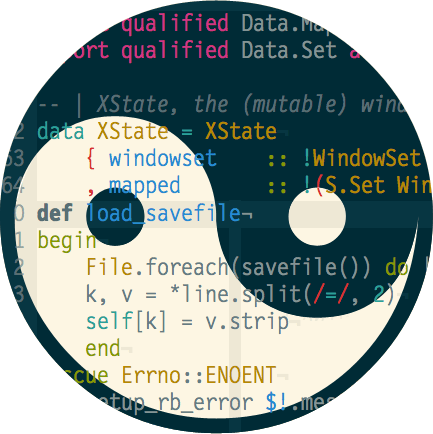
\includegraphics[width=\linewidth]{solarized-yinyang.png}
  \caption{Le thème \emph{Solarized} en sombre et en clair. \url{http://ethanschoonover.com/solarized}}
  \label{fig:solarized}
\end{marginfigure}

\begin{description}
    \item[Configuration par défaut] \vim est configurable grâce à un fichier nommé \vimrc, qui est bien entendu vide par défaut. La première étape va être d'avoir un fichier \vimrc avec une configuration minimale.
    \item[Coloration syntaxique] De base, \vim est tout blanc et tout moche. On va utiliser le thème \emph{Solarized} (\url{http://ethanschoonover.com/solarized}). Si votre but est d'être efficace, c'est le meilleur thème disponible actuellement (tout éditeur de texte confondu). La figure \ref{fig:solarized} vous donne une idée des deux look disponibles (clair ou sombre). Pour ma part j'utilise le thème sombre.
    \item[Explorateur de fichiers] Si vous utilisez \vim avec une interface graphique (ce qui est le cas de 99\% d'entre vous je suppose) vous avez par défaut un menu \Verb|Fichier| vous permettant d'ouvrir un fichier. C'est certes un bon début, mais avoir à disposition un explorateur de projet à la Netbeans ou à la Textmate peut s'avérer très pratique. Pour obtenir le même comportement, nous utiliserons Nerdtree. À savoir qu'à la fin de ce livre, vous n'aurez plus besoin de la souris (et donc des menus et autres boutons).
\end{description}

Ce chapitre est indispensable si vous n'avez que peu d'expérience (voir pas du tout) avec \vim. À la fin de ce chapitre, vous aurez un \vim dont vous pourrez commencer à vous servir pour vos tâches de tous les jours. Cela devrait être suffisant pour vous permettre d'apprendre le reste petit à petit. Car il n'y a pas de secret, il vous faudra pratiquer pour apprendre \vim, alors autant commencer de suite et le moins douloureusement possible.

En revanche, si vous êtes déjà familier avec \vim et n'utilisez déjà plus la souris, vous pouvez sagement sauter ce chapitre (soyez sur tout de même de donner sa chance au thème \emph{Solarized}).

\section{Préambule indispensable : le mode insertion}

Prenons le pari de créer le fichier \vimrc avec \vim lui même. Comme je vous le disais, le plus tôt vous commencerez, le mieux ce sera.
Vous devrez certainement commencer par installer une version de \vim. Si vous utilisez un Mac, essayez MacVim \sidenote{MacVim: \url{http://code.google.com/p/macvim/}} sans aucune hésitation. Si vous utilisez GNU/Linux ou tout autre système ``Unix'' vous devriez surement avoir gVim à votre disposition (ou tout du moins facilement installable grâce à votre gestionnaire de logiciels). Pour Windows, il semblerait y avoir une version disponible sure le site officiel de \vim\sidenote{Page de téléchargement officielle de \vim : \url{http://www.vim.org/download.php}}, mais je ne l'ai pas testée.

Cliquez sur \Verb|Fichier (File) -> Nouveau (New)|. Le texte d'accueil par défaut de \vim devrait avoir disparu et vous devriez avoir une page blanche comme sur la figure \ref{fig:vim-new}. 

\begin{figure}%
  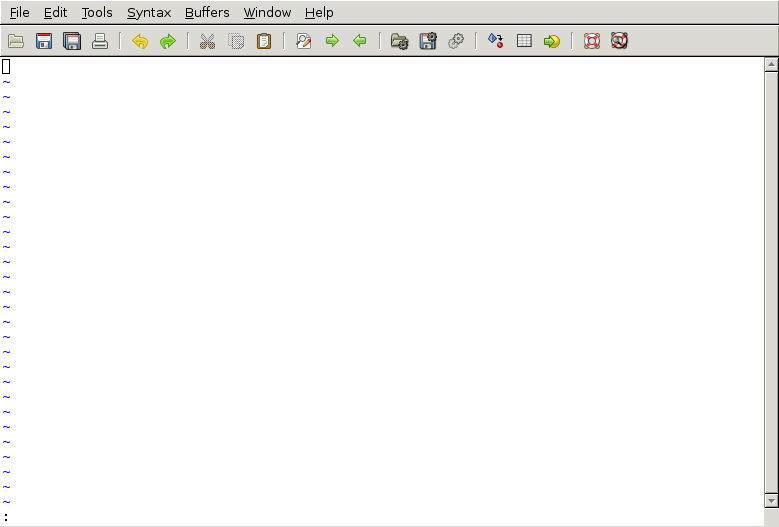
\includegraphics[width=\linewidth]{vim-new.png}
  \caption{Nouveau fichier vide.}
  \label{fig:vim-new}
\end{figure}

Commençons par entrer un commentaire dans d'entête du fichier pour y mentionner notre nom. Pour pouvoir entrer du texte appuyez sur \tti (le curseur devrait changer d'aspect) et entrez le commentaire ci-dessous\sidenote{Si vous ne savez pas trop ce que vous avez fait et que \vim vous affiche des trucs en rouge en bas à gauche au ne semble pas réagir comme il faut quand vous appuyez sur \tti, appuyez plusieurs fois sur \ttesc, ça devrait vous remettre au mode par défaut de \vim}.
\begin{listing}[H]

    \begin{minted}[bgcolor=bg, gobble=8]{vim}
        " VIM Configuration - Vincent Jousse
    \end{minted}
    \caption{Votre première ligne avec \vim.}
    \label{code:first-comment}
\end{listing}

Vous aurez remarqué que les commentaires en \emph{VimL} (le langage de configuration de \vim) commencent par un \Verb|"|. Appuyez ensuite sur \ttesc pour revenir au mode par défaut (le mode normal) de \vim. Et voilà le travail, cf figure \ref{fig:vim-first-comment}.

\begin{figure}%
  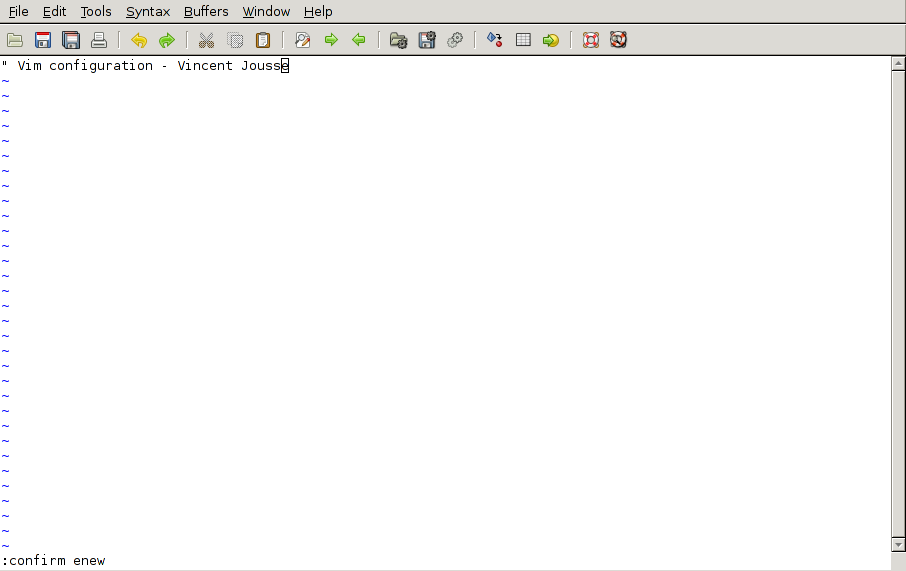
\includegraphics[width=\linewidth]{vim-first-comment.png}
  \caption{Mon premier commentaire.}
  \label{fig:vim-first-comment}
\end{figure}

Tout ça pour ça me direz vous, et vous avez bien raison. Mais tout cela a une logique que je vais vous expliquer. L'avantage de \vim est qu'il est généralement logique, quand vous avez compris la logique, tout vous semble limpide et tomber sous le sens.

Par défaut, \vim est lancé dans un mode que l'on appelle le mode ``Normal''. C'est à dire que ce mode n'est pas fait pour écrire du texte (ça, ça sera le mode ``Insert'') mais juste pour se déplacer et manipuler du texte. C'est la présence de ces 2 différents modes (il y en a d'autres mais ce n'est pas le sujet pour l'instant) qui fait toute la puissance de \vim. Il vous faudra un certain temps pour vous rendre compte de cette puissance par vous même, alors faites moi juste confiance pour l'instant.

Si vous vous demandez pourquoi ces modes, pourquoi on semble se compliquer la vie (on se la simplifie en fait) et en quel honneur, dans le mode par défaut, il n'est même pas possible d'insérer du texte, lisez attentivement la section qui suit.

\section{Les modes : d'où \vim tire sa puissance}

Je pense que nous serons tous à peu prêt d'accord sur le fait que si vous souhaitez apprendre à utiliser \vim, c'est pour gagner en efficacité pour la saisie/manipulation de texte/code. Pour gagner en efficacité lorsque l'on tape du code il n'y a pas 36 solutions, il n'y en a qu'une en fait : il faut bouger le moins possible les mains (voire pas du tout), et ne bouger que les doigts.

Pour ce faire bien sur, vous oubliez tout d'abord l'utilisation de la souris. En plus d'être lent, le mouvement clavier -> souris puis souris -> clavier est très mauvais pour vos articulations et les troubles musculosquelettiques en général\sidenote{Vous êtes peut-être jeune et n'avez pas encore eu ce type de soucis. Mais croyez moi, ça vient beaucoup plus vite qu'on ne le croit. Si vous passez votre journée sur un ordinateur, ne négligez pas ces facteurs, vous le regretterez un jour.}. D'après \emph{Wikipedia}, c'est le type de maladie professionnelle la plus courante à l'heure actuelle\sidenote{\url{https://fr.wikipedia.org/wiki/Troubles_musculosquelettiques}}.

Vous oubliez aussi le mouvement de votre main droite pour vous déplacer vers les touches directionnelles afin de bouger votre curseur. C'est une perte de temps et c'est totalement inutile avec \vim.

Qu'est-ce que vous avez le droit de faire dans le coup ? Pas grand chose, si ce n'est garder vos mains sur la position de repos comme le montre la figure \ref{fig:hand-position}. Vous trouverez d'ailleurs sur la plus part de claviers des marques sur les touches F et J, c'est pour vous donner un repère tactile d'où doivent se trouver vos indexes dans la position de repos.

\begin{figure}%
  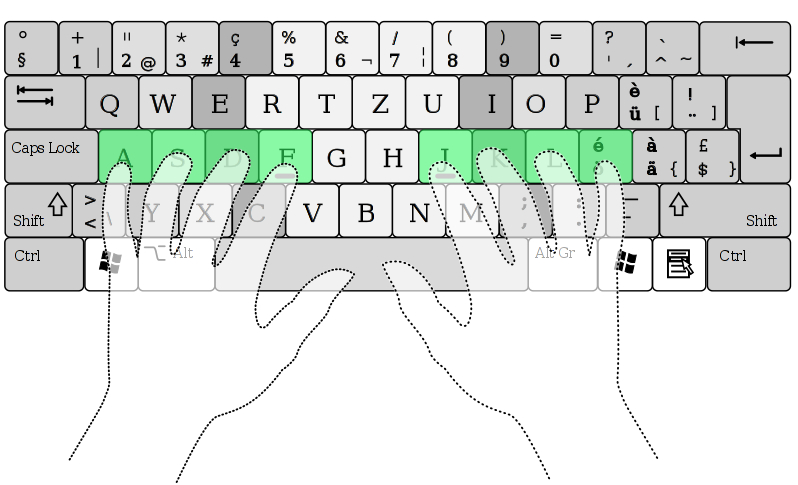
\includegraphics[width=\linewidth]{hand-position.png}
  \caption{Position de repos, clavier QWERTY. \emph{Illustration par Cy21 - CC-BY-SA-3.0 (\url{www.creativecommons.org/licenses/by-sa/3.0}) ou GFDL (\url{www.gnu.org/copyleft/fdl.html}), via Wikimedia Commons \url{http://commons.wikimedia.org/wiki/File:Typing-home-keys-hand-position.svg}}}
  \label{fig:hand-position}
\end{figure}

Ce parti pris (bouger le moins possible les mains du clavier) justifie à lui seul la présence d'un mode \emph{normal} et d'un mode \emph{insertion} dans \vim. En passant de l'un à l'autre, les touches sous vos doigts serviront tantôt à vous déplacer et à réaliser des opérations sur le texte\sidenote{C'est le mode \emph{normal}} (copier/coller, macros, \ldots), tantôt à sélectionner\sidenote{C'est le mode \emph{visuel}} et tantôt à insérer du texte\sidenote{C'est le mode \emph{insertion}}. Tout cela bien sur en évitant l'utilisation de combinaisons de touches du style \emph{Ctrl + touche} qui ne sont généralement pas bonnes pour vos doigts (\emph{Emacs} si tu nous lis, je te salue).

Par défaut, on passe du mode \emph{insertion} au mode \emph{normal} en appuyant sur la \ttesc, mais c'est une des premières choses que l'on changera : \ttesc est bien trop loin sur les claviers actuels. 

Pour passer du mode \emph{normal} au mode \emph{insertion}, on peut par exemple appuyer sur \tti On apprendra par la suite qu'il existe d'autre moyens de faire. Par exemple pour rentrer en mode insertion tout en créant une nouvelle ligne en dessous de la ligne courante (peut importe où se trouve votre curseur sur la ligne), on utilisera \tto en mode \emph{normal}.

\newthought{Si vous voulez pousser la démarche} jusqu'au bout, vous pouvez aussi vous procurer un clavier orthogonal \emph{TypeMatrix}\sidenote{\url{http://www.typematrix.com/}}. C'est ce que j'utilise personnellement, et mes doigts m'en remercient tous les jours.

\newpage
\section{La configuration par défaut : indispensable}

\newthought{Passons aux choses sérieuses}, c'est à dire comment rendre \vim un tant soit peu utilisable. Nous allons donc éditer le fichier de configuration par défaut \vimrc\sidenote{Ce fichier doit se trouver dans votre répertoire d'accueil. \emph{/home/votre\_user/.vimrc} sous Linux, \emph{/Users/votre\_user/.vimrc} sous Mac Os X ou plus généralement \emph{\textasciitilde{}/.vimrc}. Sous Windows vous pouvez créer un fichier nommé \emph{\_vimrc} qui doit se situer dans votre répertoire \emph{\%HOME\%} qui change en fonction de votre version de Windows. C'est généralement le répertoire jute "au dessus" de votre répertoire \emph{Mes Documents}. Plus d'infos sur Wikipedia \url{http://en.wikipedia.org/wiki/Home\_directory\#Default\_Home\_Directory\_per\_Operating\_System}} en y plaçant des valeurs que toute personne normalement constituée souhaiterait y voir figurer.

J'ai commenté chacune des lignes du fichier directement dans le code. Rien de sorcier ici, on se demande juste pourquoi tout cela n'est pas inclus par défaut.

\begin{listing}[H]
    \inputminted[bgcolor=bg, fontsize=\footnotesize]{vim}{../../vim-for-humans/firstconfig/vimrc}
    \caption{Une configuration par défaut sensée.}
    \label{code:first-config}
\end{listing}

J'ai mis en ligne ce fichier de configuration directement sur \emph{Github}. Vous pouvez le télécharger ou le copier directement à partir d'ici : \url{http://github.com/vjousse/vim-for-humans/fr/firstconfig/}. Il devrait aussi faire partie du package que vous avez téléchargé.

Vous devriez avoir un \vim qui ressemble à celui sur la figure \ref{fig:first-config}. Notez les numéros de ligne sur la gauche ainsi que la position du curseur en bas à droite.

\begin{figure}%
  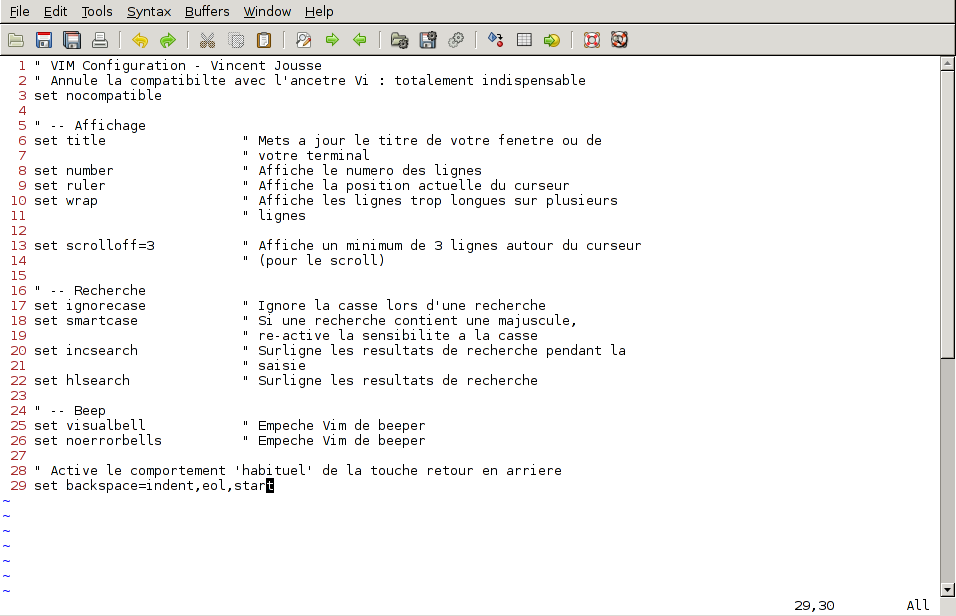
\includegraphics[width=\linewidth]{vim-first-config.png}
  \caption{\vim après votre première configuration.}
  \label{fig:first-config}
\end{figure}

Bon c'est bien beau tout ça mais ça manque un peu de couleurs. Au suivant !

\section{Que la couleur soit !}

\newthought{Tout d'abord} il faut commencer par activer la coloration syntaxique du code dans le fichier de configuration. Ajoutez ces lignes à là fin de votre fichier de configuration \vimrc.

\begin{listing}[H]
\begin{minted}[bgcolor=bg, fontsize=\footnotesize]{vim}
" Active la coloration syntaxique
syntax enable
" Active les comportements specifiques aux types de fichiers comme
" la syntaxe et l'indentation
filetype on
filetype plugin on
filetype indent on
\end{minted}
  \caption{Activation de la coloration syntaxique.}
  \label{lst:syntax-hl}
\end{listing}

Vous devriez avoir un \vim qui ressemble à celui de la figure \ref{fig:syntax-hl}\sidenote{Pour l'instant, le plus facile pour que les modifications apportées à votre \vimrc soient prisent en compte, c'est de le fermer et de le ré-ouvrir. Si vous voulez vraiment vous la jouer à la \vim de suite, en mode normal tapez \vimscmd{:so \textasciitilde/.vimrc}.

\vimscmd{:so} étant un raccourci pour \vimscmd{:source}.}. C'est une bonne première étape, passons maintenant à l'utilisation d'un thème.

\begin{figure}%
  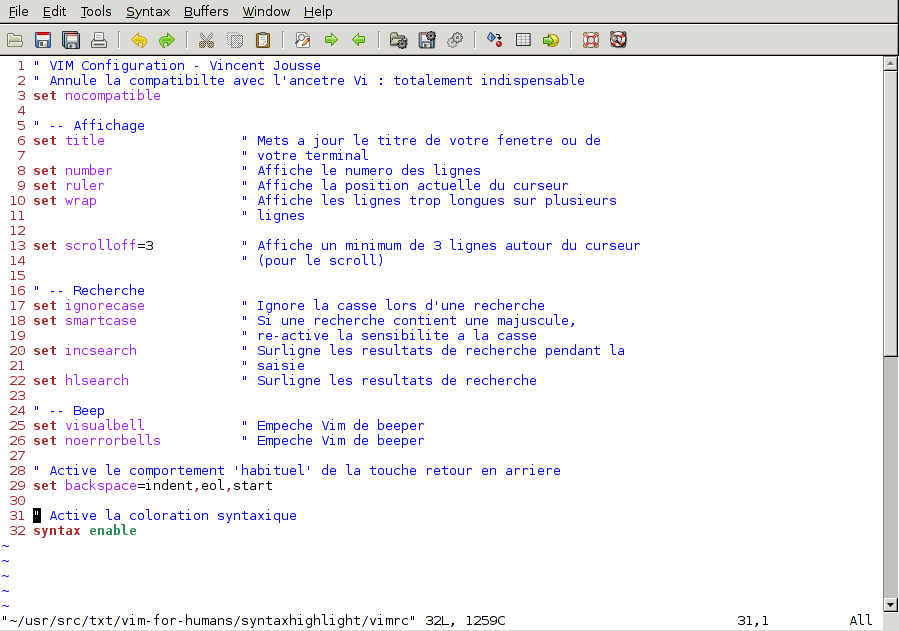
\includegraphics[width=\linewidth]{vim-syntax-hl.png}
  \caption{Coloration syntaxique par défaut.}
  \label{fig:syntax-hl}
\end{figure}

Les thèmes vont vous permettre de rendre votre \vim un peu moins austère en changeant généralement la couleur de fond ainsi que les couleurs par défaut pour le code. Comme je l'ai mentionné plus haut, nous allons utiliser le thème solarized \url{http://ethanschoonover.com/solarized} (avec fond clair ou foncé, ça dépendra de vous).

Pour l'installer, commencez tout d'abord par créer un répertoire nommé \Verb|.vim|\sidenote{Ce répertoire s'appelle \Verb|vimfiles| sous Windows. À chaque fois que je ferai référence au répertoire \Verb|.vim| ça sera en fait \Verb|vimfiles| pour les Windowsiens} au même endroit que votre \vimrc\sidenote{Dans votre répertoire utilisateur donc.}. Dans ce répertoire \Verb|.vim|, créez un sous-répertoire nommé \Verb|colors|. Téléchargez ensuite le fichier du thème Solarized \url{https://raw.github.com/altercation/vim-colors-solarized/master/colors/solarized.vim}\sidenote{ou copiez celui qui vous a été fourni avec le téléchargement de ce livre}(c'est le même fichier pour les deux versions du thème) et copiez le dans le répertoire \Verb|vim/colors/| fraichement créé. Activez ensuite le thème Solarized dans votre \vimrc comme le montre le code dans le listing \ref{lst:solarized}. Pour tester le thème clair, remplacez \Verb|dark| par \Verb|light| pour la valeur \Verb|background|.

\begin{listing}[H]
\begin{minted}[bgcolor=bg, fontsize=\footnotesize]{vim}
" Utilise la version sombre de Solarized
set background=dark
colorscheme solarized
\end{minted}
  \caption{Activation de la coloration syntaxique.}
  \label{lst:solarized}
\end{listing}

Les images \ref{fig:vim-solarized-dark} et \ref{fig:vim-solarized-light} vous donnent un aperçu des deux variantes (ma préférence allant à la variante sombre soit dit en passant).

\begin{figure}%
  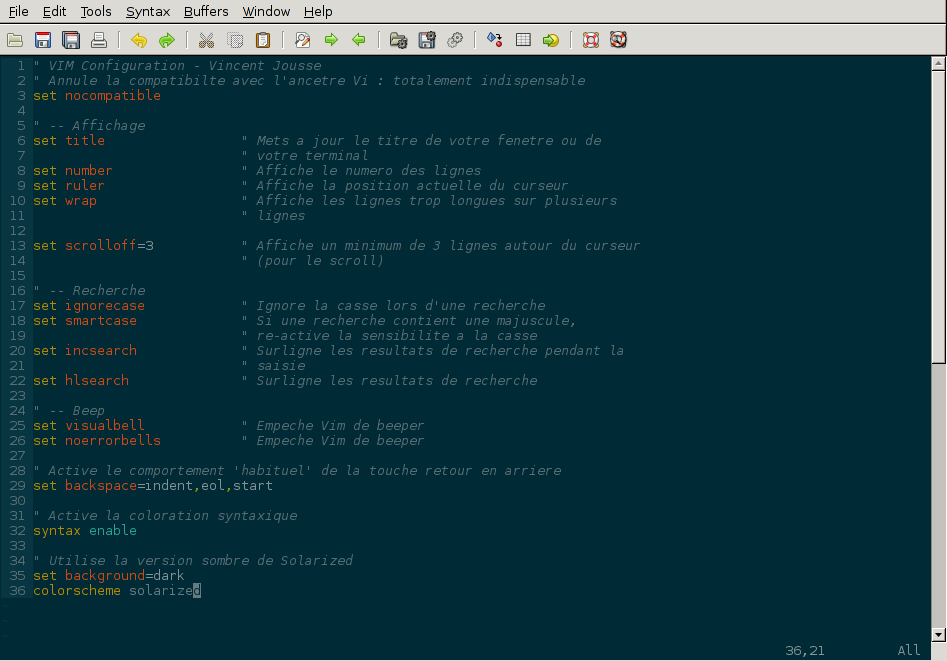
\includegraphics[width=\linewidth]{vim-solarized-dark.png}
  \caption{Le thème Solarized sombre.}
  \label{fig:vim-solarized-dark}
\end{figure}

\begin{figure}%
  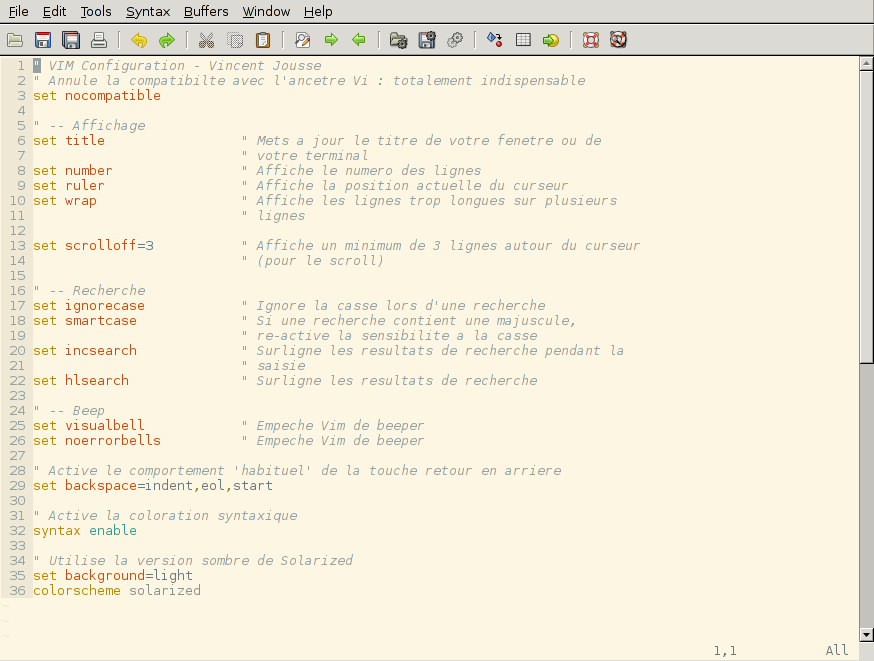
\includegraphics[width=\linewidth]{vim-solarized-light.png}
  \caption{Le thème solarized clair.}
  \label{fig:vim-solarized-light}
\end{figure}

\newthought{Un bonus} (si vous n'utilisez pas \vim directement dans votre terminal) serait de choisir une police de caractère qui vous convient un peu mieux, c'est bien sur facultatif mais bon, je présume que certains d'entre vous sont des esthètes aguerris.

Si vous êtes sous Mac Os X je vous conseille la police \Verb|Monaco| qui est plutôt sympathique. Rajoutez les lignes suivantes à votre \vimrc pour l'utiliser :

\begin{listing}[H]
\begin{minted}[bgcolor=bg, fontsize=\footnotesize]{vim}
set guifont=Monaco:h13
set antialias
\end{minted}
  \caption{Utilisation de la police Monaco sous Mac Os X.}
  \label{lst:monaco}
\end{listing}

Vous pouvez bien sur changer le \Verb|h13| par \Verb|h12| si vous voulez une police plus petite (ou par \Verb|h14| si vous en voulez une plus grande).

Sinon sous Linux j'utilise la police \Verb|DejaVu Sans Mono| que je trouve plutôt sympathique :

\begin{listing}[H]
\begin{minted}[bgcolor=bg, fontsize=\footnotesize]{vim}
set guifont=DejaVu\ Sans\ Mono\ 10
set antialias
\end{minted}
  \caption{Utilisation de la police DejaVuSansMono sous Linux.}
  \label{lst:dejavusansmono}
\end{listing}

Vous pouvez là aussi bien sur changer la taille de la police si vous le souhaitez. Pour avoir la liste des polices disponibles tapez on mode normal \vimcmd{:set guifont:*}.

Vous trouverez une version complète du fichier de configuration pour ce chapitre en ligne \url{https://github.com/vjousse/vim-for-humans/blob/master/syntaxhighlight/vimrc} ou avec les fichiers mis à disposition avec ce livre. Je ne m'attarderai pas plus sur les polices, c'est assez dépendant de votre système d'exploitation, et un peu moins de \vim dans le coup.


\section{L'explorateur de fichiers : notre premier plugin}

Nous y voilà, nous avons un \vim à peu près utilisable avec de jolies couleurs. Maintenant, il faudrait être capable d'ouvrir des fichiers autrement qu'en faisant \Verb|Fichier (File) -> Ouvrir (Open)|. Ça va être une bonne occasion pour installer notre premier plugin (ce n'est pas comme si nous avions d'autres choix de toute façon). Nous allons procéder ici en deux étapes, tout d'abord installer un gestionnaire de plugin pour éviter que ça devienne trop le bazaar dans vos plugins, puis installer ensuite le plugin qu'il nous faut pour explorer un répertoire de fichiers.

\subsection{Gestionnaire de plugins: Pathogen}

Pathogen\sidenote{\url{https://github.com/tpope/vim-pathogen/}} est typique du plugin que vous découvrez après avoir commencé à configurer votre \vim et qui génère ce type de réaction : "Ah si j'avais su j'aurais directement commencé avec". Ça tombe bien, c'est ce que nous allons faire.

Tout d'abord petite explication de comment on installe et configure des plugins dans \vim. Ils s'installent en copiant les fichiers adéquats (la plus part du temps avec une extension en \emph{*.vim}) dans des sous répertoires de votre répertoire de configuration \emph{.vim}. On a déjà d'ailleurs commencé à y créer un sous-répertoire \Verb|colors| qui contient notre "plugin" de coloration Solarized.

Le problème avec cette approche c'est que les différents plugins ne sont pas isolés (vous allez devoir copier leurs fichiers dans les différents sous-répertoires) et que vous allez donc vous retrouver avec des fichiers un peu partout sans savoir à qui ils appartiennent. Autant vous dire qu'une fois que vous voulez désinstaller ou mettre à jour un plugin, c'est vite l'enfer pour savoir quels sont ses fichiers.

C'est la que pathogen arrive à la rescousse, il va vous permettre d'installer chaque plugin dans un sous répertoire rien que pour lui. La figure \ref{fig:pathogen-tree} vous donne un exemple de répertoire \Verb|.vim| avant et après l'utilisation de pathogen. Certes la version avec pathogen contient plus de sous répertoires, mais croyez moi sur parole, ce rangement va vous éviter bien des ennuis par la suite\sidenote{Et vous pourrez au passage très facilement utiliser \emph{git} pour gérer chacun de vos plugins comme des submodules, ce qu'il est impossible de réaliser sinon.}.

\begin{figure}%
  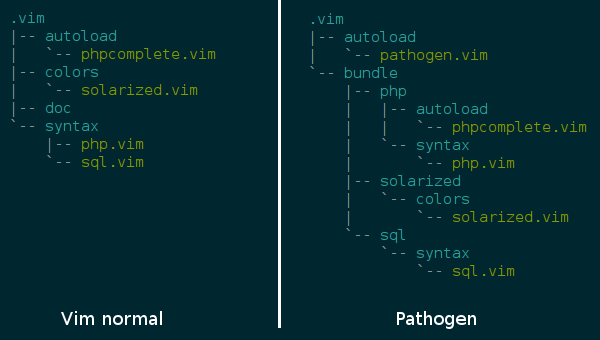
\includegraphics[width=\linewidth]{pathogen-tree.png}
  \caption{\emph{.vim} avant et après Pathogen.}
  \label{fig:pathogen-tree}
\end{figure}

Commençons par installer pathogen. Créez un répertoire nommé \Verb|autoload| dans votre répertoire \Verb|.vim| et copiez y \Verb|pathogen.vim| que vous pouvez télécharger ici : \url{https://raw.github.com/tpope/vim-pathogen/master/autoload/pathogen.vim} (ou qui vous a été fourni avec ce PDF). Pour les utilisateurs Unix, le listing \ref{code:pathogen-install} explique comment l'installer\sidenote{Si vous n'avez pas \Verb|{\footnotesize curl}| vous pouvez aussi utiliser \scmd{wget -O -}}.

\begin{listing}[H]
\begin{minted}[bgcolor=bg, fontsize=\footnotesize]{sh}
# Creation du repertoire autoload
mkdir -p ~/.vim/autoload 

# Telechargement et installation de pathogen
curl -so ~/.vim/autoload/pathogen.vim \
    https://raw.github.com/tpope/vim-pathogen/master/autoload/pathogen.vim
\end{minted}
  \caption{Installation de pathogen.}
  \label{code:pathogen-install}
\end{listing}

Nous installerons ensuite nos plugins directement dans le répertoire \Verb|.vim/bundle| que vous allez vous empresser de créer, cf. le listing \ref{code:pathogen-bundle}.

\begin{listing}[H]
\begin{minted}[bgcolor=bg, fontsize=\footnotesize]{sh}
# Creation du repertoire bundle
mkdir -p ~/.vim/bundle
\end{minted}
  \caption{Création du répertoire d'installation des plugins.}
  \label{code:pathogen-bundle}
\end{listing}

Il ne vous reste plus qu'à activer pathogen dans votre \vimrc et le tour est joué. Nous placerons le code listé dans 
\ref{code:pathogen} au début du fichier \vimrc, directement après la ligne \Verb|set nocompatible|.

\begin{listing}[H]

\begin{minted}[bgcolor=bg]{vim}
" Activation de pathogen
call pathogen#infect()
\end{minted}
\caption{Activation du plugin pathogen.}
\label{code:pathogen}
\end{listing}

Puisque charité bien ordonnée commence par soit même, nous allons ranger notre petit plugin solarized en utilisant pathogen. Il nous suffit de créer un répertoire \Verb|solarized| dans notre répertoire \Verb|bundle| fraichement créé\sidenote{Vous pouvez l'appeler comme vous le souhaitez, tout sous-répertoire du répertoire \Verb|{\footnotesize bundle}| sera considéré comme un répertoire de plugin.}. Nous déplaçons ensuite le répertoire \Verb|colors| dans le répertoire \Verb|solarized| cf. le listing \ref{code:solarized-bundle}.

\begin{listing}[H]
\begin{minted}[bgcolor=bg, fontsize=\footnotesize]{sh}
# Creation du repertoire pour solarized
mkdir ~/.vim/bundle/solarized
# Et hop un peu de rangement
mv ~/.vim/colors ~/.vim/bundle/solarized
\end{minted}
  \caption{Utilisation de solarized via pathogen.}
  \label{code:solarized-bundle}
\end{listing}

Voilà notre \vim est presque près pour le grand bain. Il vous reste une petite étape à franchir : disposer d'un moyen pratique pour explorer les fichiers d'un projet, c'est ici que \emph{The NERD Tree} entre en lisse.

\subsection{Explorateur de fichiers : The NERD Tree}

The NERD Tree est un plugin permettant d'afficher visuellement une arborescence de fichiers directement dans la partie gauche (par défaut) dans votre \vim à la \emph{TextMate}, \emph{Sublime Text} ou encore \emph{Eclipse/Netbeans}. Ce plugin n'est pas essentiel si vous souhaitez tout contrôler au clavier (je ne l'utilise plus moi même), mais est assez pratique lorsque l'on débute avec \vim.

L'alternative que nous verrons plus tard au chapitre \TODO est d'utiliser le plugin \emph{Ctrl-p} pour trouver des fichiers et les plugins \emph{LustyExplorer} et \emph{LustyJuggler} pour naviguer entre les fichiers. En effet, devoir visualiser l'arborescence pour trouver un fichier est toujours plus lent que de trouver le fichier à partir de son nom par exemple. The NERD Tree vous permettra donc d'obtenir un \vim se comportant comme un éditeur classique avec un explorateur de fichiers sur lequel vous pourrez cliquer.

Nous allons tout d'abord préparer pathogen pour installer les différents fichiers de \emph{The NERD Tree}.

\begin{listing}[H]
\begin{minted}[bgcolor=bg, fontsize=\footnotesize]{sh}
# Creation du repertoire pour The NERD Tree
mkdir ~/.vim/bundle/nerdtree
\end{minted}
  \caption{Création du répertoire pour The NERD Tree.}
  \label{code:nerdtree-bundle}
\end{listing}

Téléchargez ensuite le dernier \emph{.zip} disponible sur la page du plugin \url{http://www.vim.org/scripts/script.php?script_id=1658}. À l'heure où j'écris ces lignes la dernière version disponible est la version 4.2.0 disponible en téléchargement à cette adresse\sidenote{C'est la version que vous trouverez dans les fichiers mis à disposition avec ce PDF} : \url{http://www.vim.org/scripts/download_script.php?src_id=17123}.

Ouvrez le fichier zip et placez son contenu dans le répertoire \Verb|~/.vim/bundle/nerdtree| que nous venons de créer. Vous devriez avoir une arborescence ressemblant à celle ci-dessous pour votre répertoire \Verb|nerdtree| :

\begin{verbatim}
nerdtree
|-- doc
|   `-- NERD_tree.txt
|-- nerdtree_plugin
|   |-- exec_menuitem.vim
|   `-- fs_menu.vim
|-- plugin
|   `-- NERD_tree.vim
`-- syntax
    `-- nerdtree.vim
\end{verbatim}

Il va ensuite falloir activer le plugin. Vous pouvez le faire manuellement en tapant \vimcmd{:NERDTree} en mode normal. Si vous préférez activer \emph{The NERD Tree} à chaque fois que vous ouvrez votre \vim, ajoutez ces lignes dans votre \vimrc:

\begin{listing}[H]
\begin{minted}[bgcolor=bg]{vim}
" Activation de NERDTree au lancement de vim
autocmd vimenter * NERDTree
\end{minted}
\caption{Activation de NERDTree au lancement de \vim.}
\label{code:pathogen}
\end{listing}

Rien de particulier ensuite, \emph{The NERD Tree} vous affiche l'arborescence du répertoire où vous avez lancé \vim, comme vous le montre la figure \ref{fig:vim-nerdtree}. Vous pouvez utiliser la souris et/ou le clavier pour vous déplacer. 

Vous pouvez aussi effectuer des commandes (créer, copier des fichiers) en appuyant sur \ttm lorsque vous êtes dans \emph{The NERD Tree}. Pour passer de la fenêtre de \emph{NERD Tree} à la fenêtre d'édition de votre fichier au clavier, appuyez sur \hlred{Ctrl + w + w}\sidenote{La touche \hlred{\emph{Control}} (Ctrl) et tout en la laissant appuyée, deux fois \hlred{w}.}. Ce raccourci clavier sera d'ailleurs toujours valable pour naviguer entre vos différentes fenêtres \vim (il n'est pas spécifique à \emph{The NERD Tree}).

\begin{figure}%
  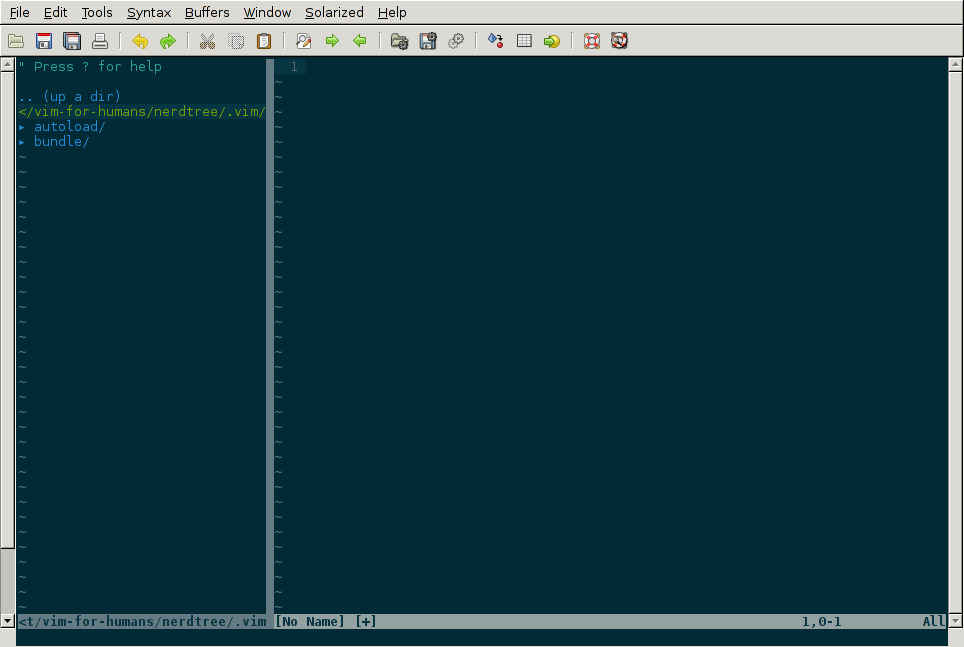
\includegraphics[width=\linewidth]{vim-nerdtree.png}
  \caption{\emph{.vim} avec \emph{The NERD Tree} d'activé.}
  \label{fig:vim-nerdtree}
\end{figure}



\chapter{L'outil de manipulation de texte rêvé}

Alors oui, pour ceux qui se demandent, je fais des rêves bizarres, mais bon chacun a ses petites tares cachées. Et rêver d'un outil qui améliore ma vie quotidienne en tant que codeur n'est pas si étrange que ça.

Ce qui fait et fera encore le succès de \vim est sa capacité à faciliter les manipulations de texte. Certes il va vous proposer des fonctionnalités propres à chaque tâche que vous effectuerez \footnote{Souvent par l'intermédiaire de plugin.} comme la validation syntaxique de code, la correction orthographique, \ldots Mais à la fin, c'est toujours à écrire/corriger/manipuler/se déplacer dans du texte que vous passerez la majeure partie de votre temps. 

C'est la que l'approche de \vim est différente d'IDE comme Eclipse / Netbeans / PhpStorm/\ldots Là où ces IDE vont mettre l'accent sur les particularités de votre langage de programmation tout en vous fournissant des capacités de manipulation de texte basiques, \vim adopte l'approche opposée : vous serez très efficace à manipuler/écrire du texte quelque soit le texte et vous pourrez enrichir \vim avec des fonctionnalités propres à votre langage de programmation via des.

Nous allons donc voir dans ce chapitre comment utiliser \vim à bon escient (vous allez commencer à oublier votre souris) et quelle est la logique derrière tout cet enchaînement de commandes qui paraissent barbare au non initié. Vous devriez pouvoir, à la fin de ce chapitre, vous passer de votre souris pour éditer/manipuler le contenu d'un fichier.

\chapter{Les plugins indispensables}

\printindex

\end{document}
